% Latex template: mahmoud.s.fahmy@students.kasralainy.edu.eg
% For more details: https://www.sharelatex.com/learn/Beamer

\documentclass[aspectratio=1610]{beamer}					% Document class

\setbeamertemplate{footline}[text line]{%
  \parbox{\linewidth}{\vspace*{-8pt}Interferon-$\gamma$ induction in HeLa cells \hfill\insertshortauthor\hfill\insertpagenumber}}
\setbeamertemplate{navigation symbols}{}

\usepackage[english]{babel}				% Set language
\usepackage[utf8x]{inputenc}			% Set encoding

\mode<presentation>						% Set options
{
  \usetheme{default}					% Set theme
  \usecolortheme{default} 				% Set colors
  \usefonttheme{default}  				% Set font theme
  \setbeamertemplate{caption}[numbered]	% Set caption to be numbered
}

% Uncomment this to have the outline at the beginning of each section highlighted.
%\AtBeginSection[]
%{
%  \begin{frame}{Outline}
%    \tableofcontents[currentsection]
%  \end{frame}
\usepackage{graphicx}					% For including figures
\usepackage{booktabs}					% For table rules
\usepackage{hyperref}	
\usepackage{tikz-network}				% For cross-referencing
\usepackage[absolute,overlay]{textpos}
\usepackage{bm}
\usepackage[font=small,labelfont=bf]{caption}				% For cross-referencing

\title{Interferon-$\gamma$ induction in HeLa cells}	% Presentation title
\author{Clayton W. Seitz}								% Presentation author
\date{\today}									% Today's date	

\begin{document}

% Title page
% This page includes the informations defined earlier including title, author/s, affiliation/s and the date
\begin{frame}
  \titlepage
\end{frame}


% The following is the most frequently used slide types in beamer
% The slide structure is as follows:
%
%\begin{frame}{<slide-title>}
%	<content>
%\end{frame}

\begin{frame}
Stepping stone project towards highly multiplexed FISH imaging
\end{frame}


\begin{frame}{The principle of Interferon-$\gamma$ induced transcriptional memory}
\begin{figure}
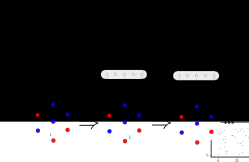
\includegraphics[width=14cm]{figure-1.png}
\caption{}
\end{figure}

Siwek et al. \textit{Activation of Clustered IFNg Target Genes Drives Cohesin-Controlled Transcriptional Memory}. Molecular Cell 2020

\end{frame}


\begin{frame}{Total RNA-seq identifies GBP5 as a memorized gene}
\begin{figure}

\includegraphics[width=13cm]{figure-2.png}
\end{figure}

\end{frame}

\begin{frame}{Single-cell RNA-seq identifies GBP5 as a memorized gene}
\begin{figure}

\includegraphics[width=12cm]{figure-3.png}
\end{figure}

\end{frame}

\begin{frame}{BLASTing probes for GPB5 and CD274}
Probes are designed against the sequence of splicing variant 1
\vspace{0.5in}
\begin{itemize}
\item{What fraction of 48 probes designed for a particular gene bind to a transcript variant of the target gene other than variant 1?}
\item{What fraction of 48 probes designed for a particular gene bind to 1 or more off target transcripts with E-value less than 0.05?}
\item{Each off-target hit will have a number (out of 48) probes that will bind to it. What is the distribution of that number over all off target hits?}
\end{itemize}
\end{frame}

\begin{frame}{BLASTing probes for GPB5 and CD274}

\end{frame}



\end{document}